% WACV 2027 submission — proposal / short paper.
% Review (double-blind) version is active below; to reveal authors for a
% camera-ready or course draft, comment the [review,...] line and uncomment
% \usepackage{wacv}.
\documentclass[10pt,twocolumn,letterpaper]{article}

\usepackage[review,applications]{wacv}      % REVIEW version (Applications track)
% \usepackage{wacv}                          % CAMERA-READY (shows authors)

%
% Additional packages (imported before hyperref, per the WACV template).
%
\usepackage{amsmath,amssymb}
\usepackage{booktabs}
\usepackage{enumitem}
\usepackage{graphicx}
\usepackage{multirow}
\usepackage{tikz}
\usetikzlibrary{arrows.meta,positioning,shapes.geometric,fit}

%
% --- inline annotations
%
\newcommand{\red}[1]{{\color{red}#1}}
\newcommand{\todo}[1]{{\color{red}#1}}
\newcommand{\TODO}[1]{\textbf{\color{red}[TODO: #1]}}


\definecolor{wacvblue}{rgb}{0.21,0.49,0.74}
\usepackage[pagebackref,breaklinks,colorlinks,allcolors=wacvblue]{hyperref}

\def\wacvPaperID{*****} % *** Enter the WACV Paper ID here for the review version
\def\confName{WACV}
\def\confYear{2027}

\title{Label-Efficient Dark-Vessel Detection in SAR:\\
Does SAR-Domain Pretraining Beat Optical and ImageNet Transfer Across ViT and CNN?}

\author{John Roth \qquad Kyle Wagner\\
Johns Hopkins University\\
{\tt\small jroth32@jh.edu \qquad kwagne35@jh.edu}
}

\begin{document}
\maketitle

\begin{abstract}
Detecting vessels without an Automatic Identification System correlate
(dark vessels) in spaceborne synthetic aperture radar (SAR) is operationally
important, yet human-verified labels are scarce. We study how pretraining
domain affects label efficiency on xView3-SAR~\cite{paolo2022xview3} under one
fixed point-native detector. Two size-matched tracks---ViT-B/16
($\sim$86M parameters) and ConvNeXt-V2-Base ($\sim$89M)---each compare random,
generic ImageNet-1K, optical remote-sensing, and SAR initialization at nested
10/25/50/100\% scene-level training fractions. Within each track,
architecture, input, detector, optimization, and the fixed run seed (0) are
held constant; only encoder initialization changes. All six pretrained
encoders are exact downloaded checkpoints, and this project performs no
backbone pretraining. The controlled matrix contains 32 seed-0 fine-tunes;
two external references are reported separately. We report detection-F1 label-efficiency curves as
point estimates, near-shore F1, and---on a disjoint, once-touched 50-scene
verified set---dark-vessel recall. Differences in pretraining objective and
history are stated explicitly when interpreting domain and architecture gaps.
\end{abstract}

\section{Introduction}
\label{sec:intro}
Detecting ships without an Automatic Identification System (AIS)
correlate---dark vessels---in spaceborne SAR is a critical maritime-monitoring
problem with scarce labels. xView3-SAR~\cite{paolo2022xview3} provides
Sentinel-1 imagery, but its human-verified dark-vessel examples are limited to
a small held-out set.

Pretrained backbones can help, but it is unclear which source transfers best:
generic natural images (ImageNet-1K~\cite{deng2009imagenet}), optical remote
sensing (fMoW-RGB~\cite{christie2018fmow} via
SatDINO~\cite{straka2025satdino}, or BigEarthNet-S2), or SAR imagery (SAR-1M
via SARMAE~\cite{liu2026sarmae}, or BigEarthNet-S1)---and whether the answer is
the same for a ViT~\cite{dosovitskiy2021image} and a
ConvNeXt~\cite{woo2023convnextv2}. We compare exact released checkpoints
rather than pretraining our own, avoiding a confound from locally chosen
source-training recipes~\cite{zoph2020rethinking}. The released checkpoints
are not all method-matched, so pretraining objective and history remain
explicit interpretation limits rather than hidden assumptions.

With the detector, schedule, and input fixed, we ask:
\textbf{(Q1)} how much labeled xView3 data does each initialization save
relative to random initialization to reach a target overall detection F1;
\textbf{(Q2)} does SAR-domain pretraining beat both optical remote-sensing and
generic ImageNet transfer in the scarce-label regime; and \textbf{(Q3)} is any
such advantage \emph{architecture-general}, holding for both a ViT and a
size-matched CNN? We hypothesize that SAR initialization yields the largest
low-label gain over the random floor in both tracks. Because the approved
study uses seed 0 only, its curves are descriptive point estimates, not
variance or significance estimates.

\section{Approach}
\label{sec:approach}

\paragraph{Design.} The study has two architecture-matched tracks---ViT-B/16
($\sim$86M) and ConvNeXt-V2-Base ($\sim$89M, deliberately size-matched)---each
with four arms that share the same head, optimizer, schedule, and fixed seed
0; only the downloaded initialization differs (Table~\ref{tab:arms}).
Initialization is the only variable within a track and architecture the only
variable across matched roles. Comparing arm $k$ to arm $k{+}4$ holds the
pretraining role fixed while changing architecture, subject to the disclosed
cross-track training-history differences.

\begin{table*}[t]
\centering
\small
\setlength{\tabcolsep}{5pt}
\begin{tabular}{@{}cllllcl@{}}
\toprule
\textbf{Arm} & \textbf{Track} & \textbf{Backbone} & \textbf{Initialization} & \textbf{Params} & \textbf{On curve?} & \textbf{Role} \\
\midrule
1 & ViT & ViT-B/16 & random init & $\sim$86M & yes & ViT floor \\
2 & ViT & ViT-B/16 & SatDINO (fMoW-RGB, DINO) & $\sim$86M & yes & optical-domain transfer \\
3 & ViT & ViT-B/16 & SARMAE (SAR-1M, MAE) & $\sim$86M & yes & SAR-domain transfer \\
4 & ViT & ViT-B/16 & ImageNet-1K AugReg & $\sim$86M & yes & generic ImageNet transfer \\
5 & CNN & ConvNeXt-V2-B & random init & $\sim$89M & yes & CNN floor \\
6 & CNN & ConvNeXt-V2-B & BigEarthNet-S2 (optical RS) & $\sim$89M & yes & optical-domain transfer \\
7 & CNN & ConvNeXt-V2-B & BigEarthNet-S1 (SAR RS) & $\sim$89M & yes & SAR-domain transfer \\
8 & CNN & ConvNeXt-V2-B & ImageNet-1K FCMAE$\rightarrow$FT & $\sim$89M & yes & generic ImageNet transfer \\
\addlinespace
R2 & ref & YOLO26 & COCO-pretrained & external & no & detector reference \\
R3 & ref & LocateAnything-3B & zero-shot & $\sim$3B & no & VLM reference \\
\bottomrule
\end{tabular}
\caption{Eight controlled arms in two size-matched tracks ($\sim$86M vs.\
$\sim$89M), plus two external references reported off the curves. Optical
anchors are SatDINO~\cite{straka2025satdino} (ViT) and
BigEarthNet-S2~\cite{clasen2025reben} (CNN); SAR anchors are
SARMAE~\cite{liu2026sarmae} (ViT) and BigEarthNet-S1~\cite{clasen2025reben}
(CNN). Both ImageNet encoders are downloaded; Arm~4 uses supervised AugReg
while Arm~8 uses FCMAE followed by supervised ImageNet-1K fine-tuning.}
\label{tab:arms}
\end{table*}

\paragraph{Initialization regimes.} The four matched roles are a random floor,
generic natural-image transfer, optical remote-sensing transfer, and SAR
transfer. The BigEarthNet-S2/S1 CNN pair provides the cleanest domain contrast:
architecture, dataset, and supervised land-cover task are shared, while
sensing modality differs. The ViT comparison is best-available rather than
method-matched because SatDINO uses DINO~\cite{caron2021emerging} and SARMAE
uses masked autoencoding~\cite{he2022masked}. The ImageNet pair shares its
final dataset and classification supervision, but not its full history: the
ViT uses supervised AugReg~\cite{steiner2021trainvit}, whereas ConvNeXt-V2 uses
FCMAE followed by supervised ImageNet-1K fine-tuning.

\paragraph{Detector.} xView3 labels are points and its metric matches
predictions by distance, not box IoU, so we use a point-native heatmap head in
the style of CenterNet / \emph{Objects as Points}~\cite{zhou2019objects}: each
vessel is a Gaussian blob on a stride-4 map, decoded by peak-finding with
distance-based non-maximum suppression. Every arm receives the same fixed
3-channel input $[\mathrm{VH},\mathrm{VV},\mathrm{VH}{-}\mathrm{VV}]$ in dB, so
input handling is never a confound between arms.

\paragraph{Fine-tuning and comparability.} All arms fine-tune end-to-end
through one code path with shared AdamW, augmentation, and seed 0. Training
runs for up to 50 epochs with early stopping on dev-split F1; the decision
threshold is selected on dev and frozen before test. Continuous-integration
guard tests make comparability a checked invariant rather than a claim: a
backbone-parity test asserts identical within-track parameter counts and
matching head-adapter geometry, a checkpoint-load test asserts that each
pretrained backbone loads exact non-random weights, and a
scorer-immutability test freezes the evaluation code
(Figure~\ref{fig:pipeline}).

\begin{figure}[t]
\centering
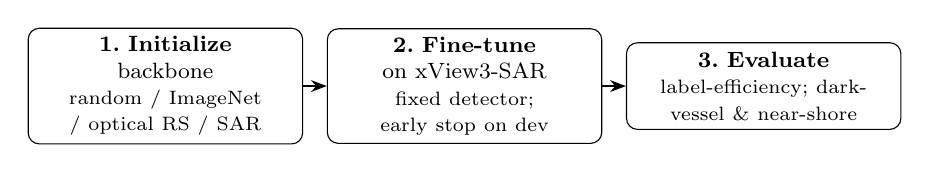
\begin{tikzpicture}[
  box/.style={draw, rounded corners, align=center, inner sep=3pt,
    font=\footnotesize, minimum height=11mm, text width=0.27\linewidth},
  arr/.style={-{Stealth[length=2mm]}, thick}
]
\node[box] (a) {\textbf{1.\ Initialize}\\ backbone\\
  {\scriptsize random / ImageNet / optical RS / SAR}};
\node[box, right=3mm of a] (b) {\textbf{2.\ Fine-tune}\\ on xView3-SAR\\
  {\scriptsize fixed detector; early stop on dev}};
\node[box, right=3mm of b] (c) {\textbf{3.\ Evaluate}\\
  {\scriptsize label-efficiency; dark-vessel \& near-shore}};
\draw[arr] (a) -- (b);
\draw[arr] (b) -- (c);
\end{tikzpicture}
\caption{The three stages, run identically for every arm; only the backbone
initialization varies within a track.}
\label{fig:pipeline}
\end{figure}

\section{Data and Evaluation}
\label{sec:data}
We use locally acquired xView3 DIU-format Sentinel-1 GRD archives with dual
polarization VH/VV. The frozen seed-0 split contains 150 study scenes: 111
train, 23 dev, and 16 test. Training fractions are nested and selected at the
scene level (10/25/50/100\%), preventing chip leakage between splits. A
separate set of exactly 50 human-verified scenes forms
\texttt{eval\_final}; it is evaluated once, after the grid and operating
thresholds are frozen, with no subsequent tuning. Dark-vessel labels occur
only in this verified set, so dark-vessel recall is not reported on dev or
test. LS-SSDD is not consumed by the active study. The controlled grid reports
eight seed-0 detection-F1 curves as point estimates, with near-shore F1 and
once-only final dark-vessel recall. YOLO26~\cite{jocher2026yolo26} and
LocateAnything-3B are the only external references and remain off the curves.

\section{Timeline and Feasibility}
\label{sec:timeline}
All six pretrained initializations are downloaded, so local training is
limited to 32 seed-0 xView3 detector fine-tunes; with the two completed
external references, the full plan contains 34 experiments. Six core
10\%-fraction cells and both references are complete, leaving 26 core cells.
Completed RTX 5070 Ti timings project roughly 19--22 days of continuous
single-GPU execution for those cells, excluding data transfer and final
evaluation. The historical V100 forecast is retired, and measured P100
throughput failed the project's compute tripwire; the remaining
recipe-identical one-GPU jobs are assigned to the RTX 5070 Ti. We target the
WACV~2027 Round-2 deadline (paper registration August~21, 2026; submission
August~28, 2026, AoE).

{
    \small
    \bibliographystyle{ieeenat_fullname}
    \bibliography{proposal}
}

\end{document}
